\chapter{Results}

This chapter presents the major results of this thesis. First, an optimal blending pattern for simultaneous crossline sources will be derived. Then, the advantages of a 3D $f$-$k_x$-$k_y$-filter towards a 2D $f$-$k$-filter will be shown. Finally, the feasibility of the suggested acquisition design will be proven on a synthetic 3D data set. 

 
\section{Blending pattern}


\begin{itemize}
	\item Explain how the acquisition limits the firing pattern
	\item Introduce spatial incoherency
	\item Suggest the applied blending pattern
	\item Show quality factor versus incoherency/firing pattern
\end{itemize}

An incoherent blending pattern is crucial for good deblending performance (see section \ref{sec:BlendingMatrix}). Thus, a measure of incoherency will be introduced. Then, the importance of the maximum firing delay time will be demonstrated.

\subsection*{Incoherency Measure}

In this thesis only the incoherency of the acquisition design is considered. Thus, the blending matrix, $\Gamma$, determines the incoherency. In section \ref{sec:BlendingMatrix} it was shown that for an incoherent blending pattern the elements, $\mathrm{e}^{-j \omega \Delta t_{kl}}$, along a sub-diagonal of the product $\mathbf{\Gamma \Gamma}^H$ should be out of phase. 

These sub-diagonal elements, $\mathrm{e}^{-j \omega \Delta t_{kl}}$, are complex numbers with unit length and variable phase. Hence, the elements are located in the complex plane on a circle with radius 1 (see Figure \ref{fig:Ch-Results-complex-circle}). 

\begin{figure}
	\centering
	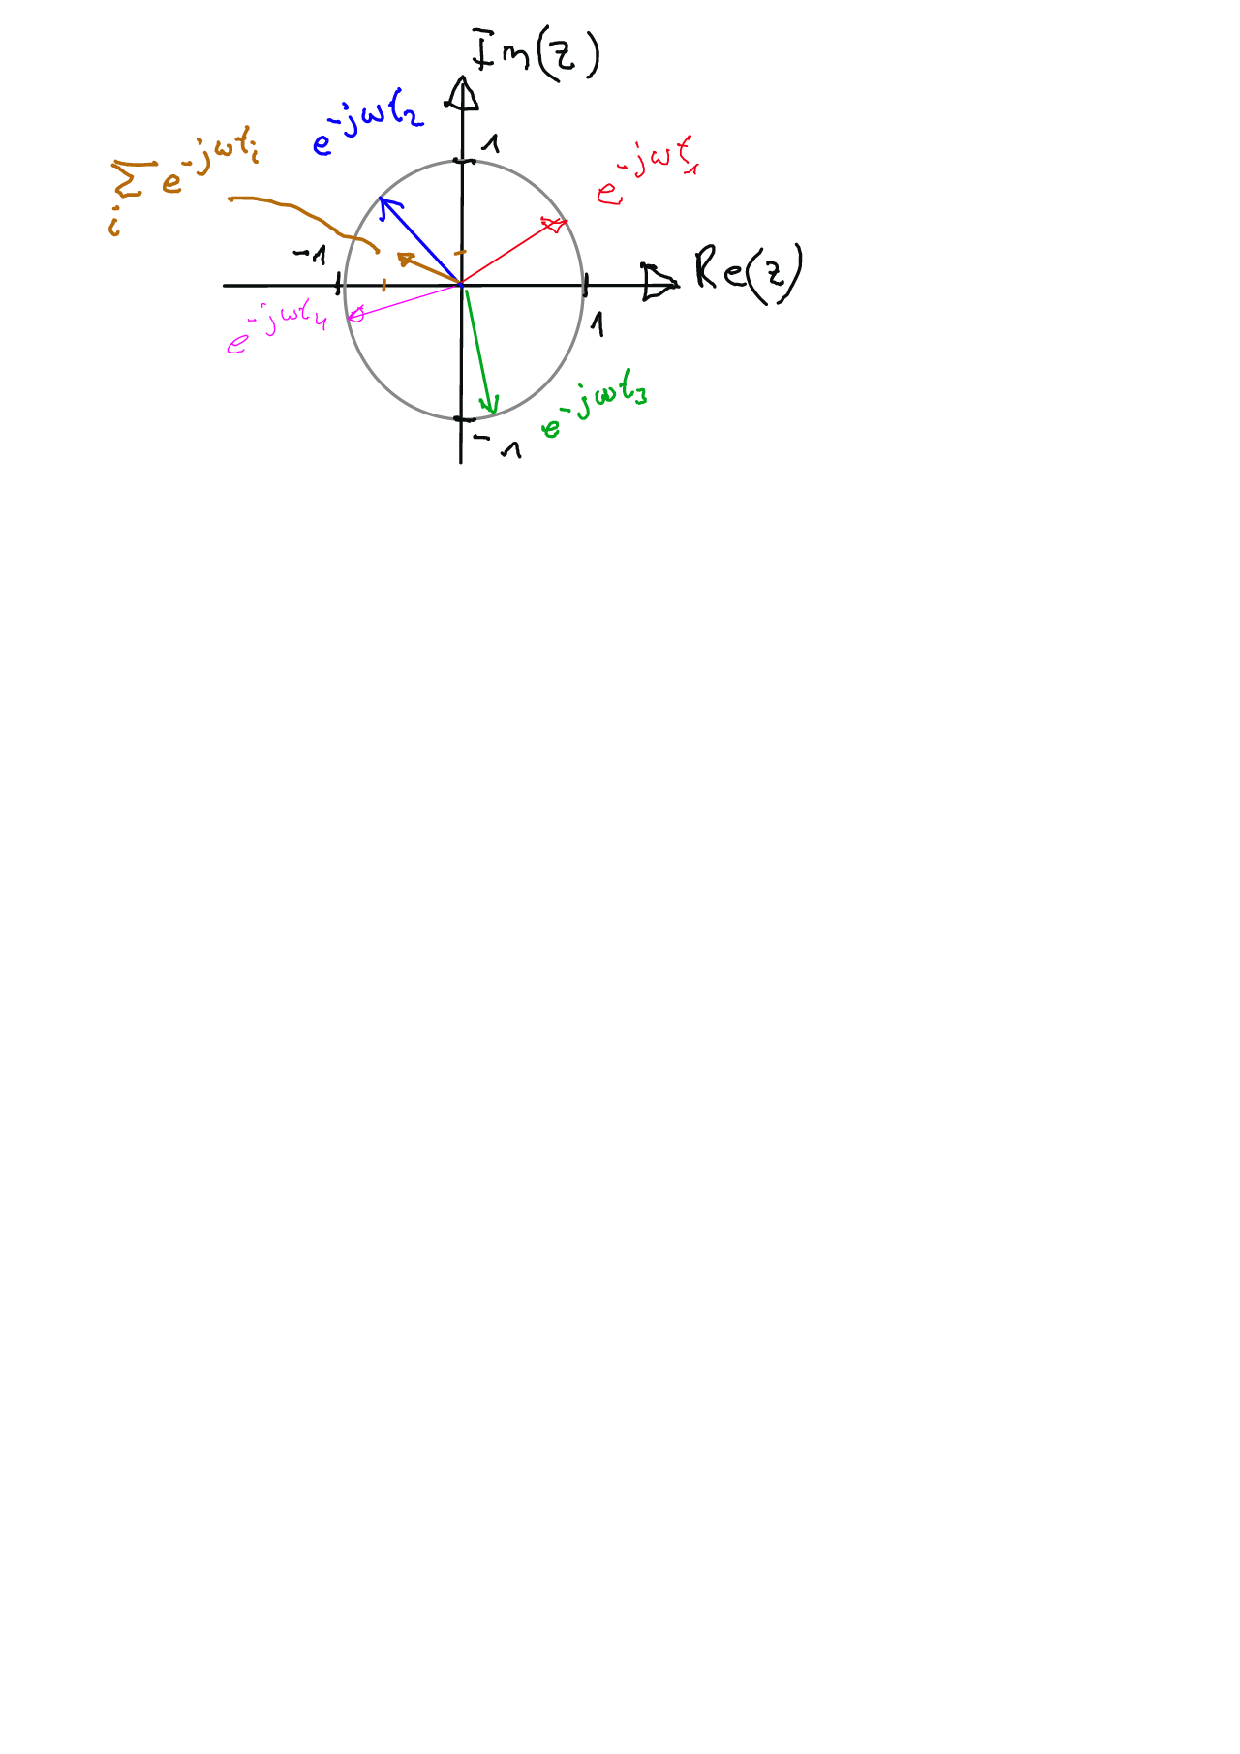
\includegraphics[width = 0.5\textwidth]{Plots/complex-circle}
	\caption{Illustration of the sub-diagonal elements in the complex number plane. The elements have unit length and variable phase. The absolute value of their sum depends on the phase coherency of the elements.}
	\label{fig:Ch-Results-complex-circle}
\end{figure}


If all elements are in phase the length of their sum is maximized. The more the elements are out of phase, i.e. the more incoherent they are, the smaller is the length of the summed elements. Figure \ref{fig:Ch-Results-Diagonal-Sums} illustrates the length of the summed sub-diagonals. The elements on the main diagonal of the product $\mathbf{\Gamma \Gamma}^H$ are all equal to 1. Thus, the spike in Figure \ref{fig:Ch-Results-Diagonal-Sums} refers to the main diagonal of $\mathbf{\Gamma \Gamma}^H$. For a perfectly incoherent blending design the elements on a sub-diagonal cancel and the plot becomes a perfect spike. 


\begin{figure}
	\centering
	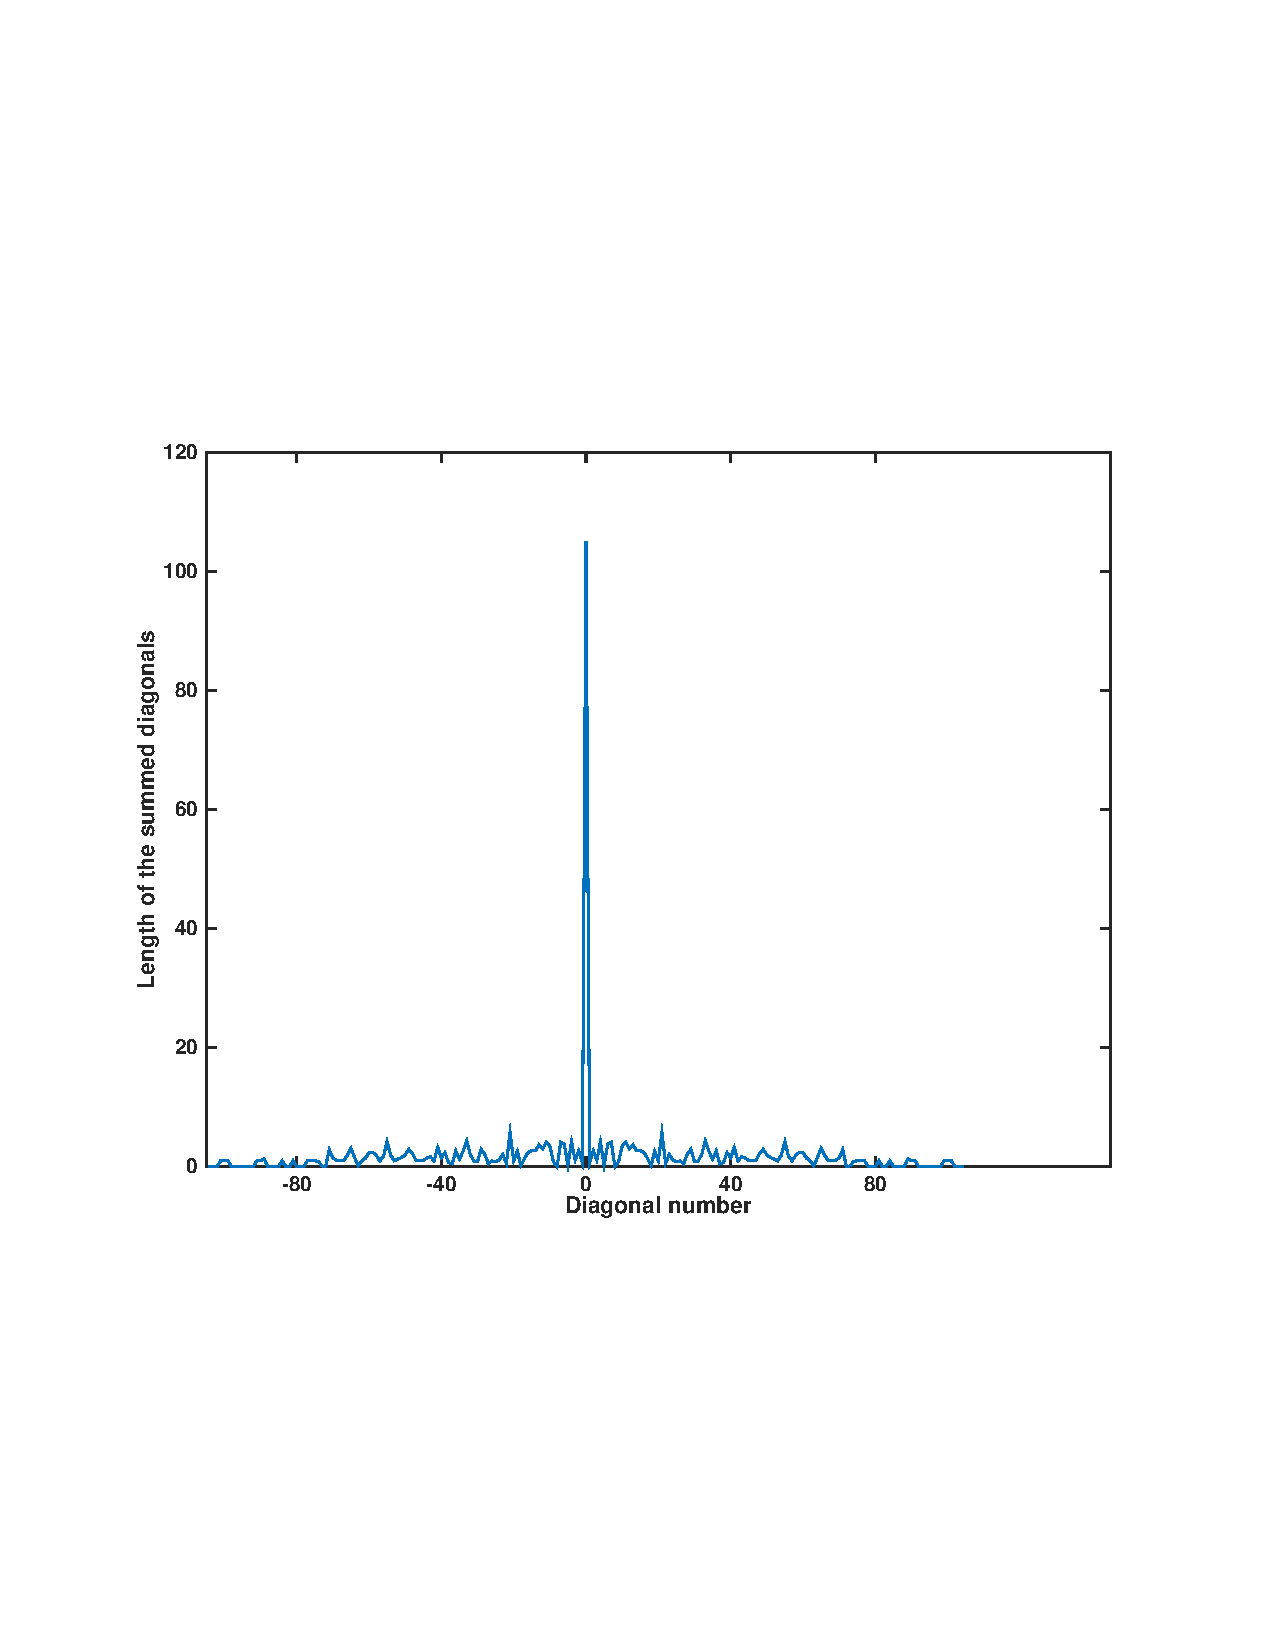
\includegraphics[width=0.6\textwidth]{Plots/diagonal-sums}
	\caption{The sub-diagonal elements, $\mathrm{e}^{-j \omega \Delta t_{kl}}$, of the product $\mathbf{\Gamma \Gamma}^H$ are summed. The length of each output is plotted as a function of the diagonal. The spike is caused by the main diagonal elements of $\mathbf{\Gamma \Gamma}^H$ because they are all in phase.}
	\label{fig:Ch-Results-Diagonal-Sums}
\end{figure}









Different incoherent blending patterns will be tested, in particular, temporally and spatially incoherent blending patterns. 

This thesis considers the following blended acquisition set up: The sources are assembled in crossline direction and move in inline direction due to the vessel movement (see Figure \ref{fig:Ch-Theory-3D-BlendedAcquisition}). As a consequence each experiment can blend sources which belong to the same crossline. The source sampling rate in inline direction must be sufficiently small to avoid spatial aliasing. Thus, the sources within one crossline must be blended and recorded before the vessel reaches the next inline position.

Based on this set up there are three possibilities to blend the sources incoherently. First, the sources can be blended with random time delays (temporal incoherency). Second, one can randomly pick sources for each experiment (spatial incoherency). Third, temporal and spatial incoherency can be combined, i.e. randomly picked sources are blended with random time delays.

In the following these blending patterns will applied to a synthetic data set (see Figure \ref{fig:Ch-Results-Unbl-Delphi}, \ref{fig:Ch-Results-Unbl-inline10}, \ref{fig:Ch-Results-Unbl-xline10}). Next, the data is deblended with the 3D deblending algorithm of section \ref{sec:MahdadMethod3d}. 

The deblending results are shown in Figure \ref{fig:Ch-Results-Debl-Delphi} and \ref{fig:Ch-Results-Debl-x-inline}. The results suggest that only spatial incoherency is not sufficient to deblend the data (see Figure \ref{fig:Ch-Results-Debl-Delphi-x}, \ref{fig:Ch-Results-Debl-inline10-x}, \ref{fig:Ch-Results-Debl-xline10-x}). By introducing random firing time delays the deblended data improves significantly as shown in Figure \ref{fig:Ch-Results-Debl-Delphi-t}, \ref{fig:Ch-Results-Debl-inline10-t}, \ref{fig:Ch-Results-Debl-xline10-t}). A combination of both spatial and temporal incoherency enhances the deblended data further (see Figure \ref{fig:Ch-Results-Debl-Delphi-xt}, \ref{fig:Ch-Results-Debl-inline10-xt}, \ref{fig:Ch-Results-Debl-xline10-xt}).

\begin{figure}
	\centering
	\begin{subfigure}[t]{0.8\textwidth}
		\centering
		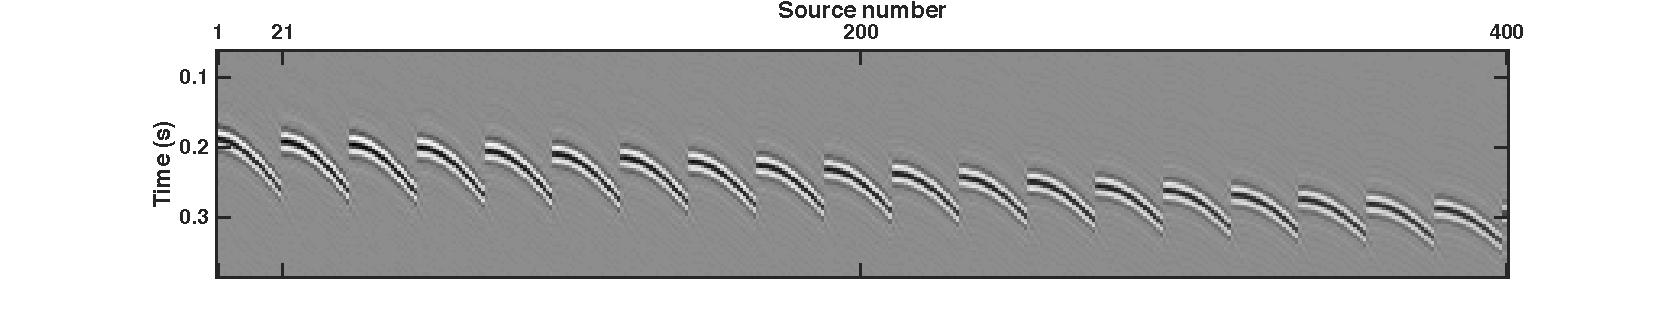
\includegraphics[width = \textwidth]{Plots/BlendingPatterns/Unblended_Delphi_zoom}
		\caption{}
		\label{fig:Ch-Results-Unbl-Delphi}
	\end{subfigure}
	\par\bigskip
	\centering
	\begin{subfigure}[t]{0.8\textwidth}
		\centering
		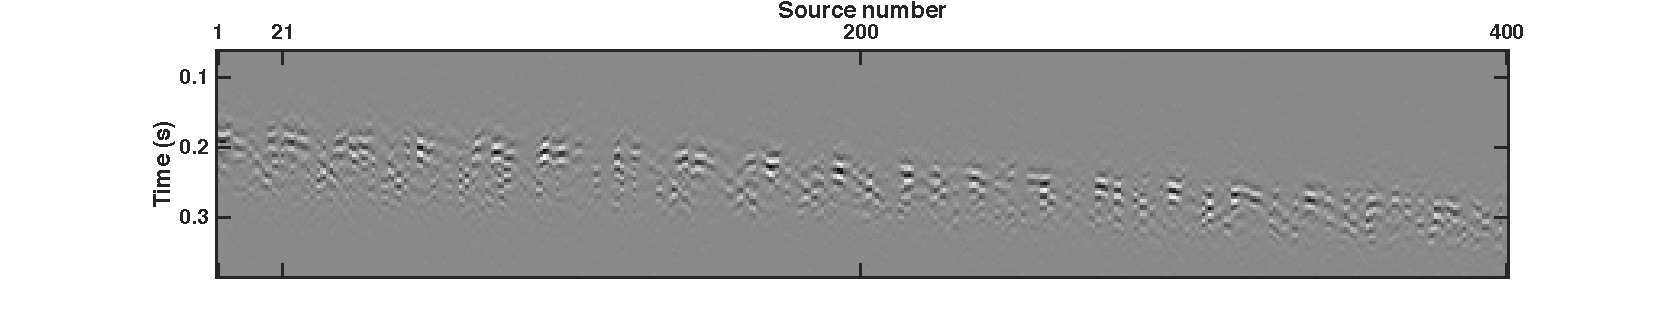
\includegraphics[width = \textwidth]{Plots/BlendingPatterns/Deblended_Delphi_zoomx}
		\caption{}
		\label{fig:Ch-Results-Debl-Delphi-x}
	\end{subfigure}
	\par\bigskip
	\centering
	\begin{subfigure}[t]{0.8\textwidth}
		\centering
		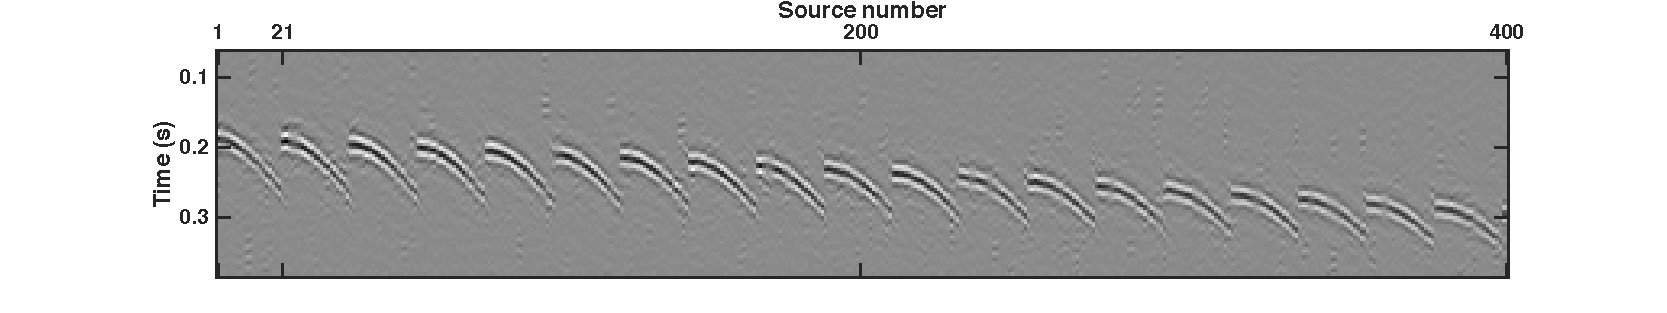
\includegraphics[width = \textwidth]{Plots/BlendingPatterns/Deblended_Delphi_zoomt}
		\caption{}
		\label{fig:Ch-Results-Debl-Delphi-t}
	\end{subfigure}
	\par\bigskip
	\centering
	\begin{subfigure}[t]{0.8\textwidth}
		\centering
		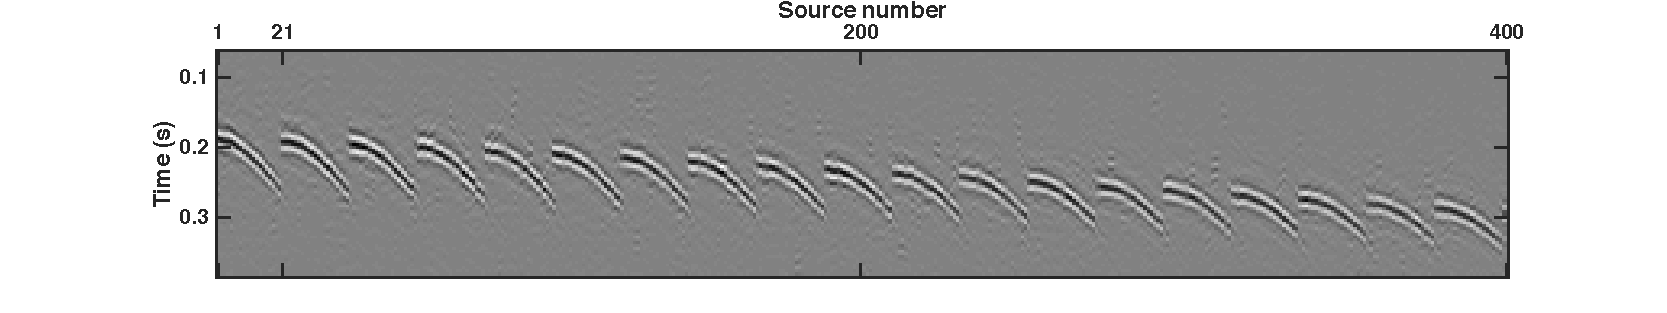
\includegraphics[width = \textwidth]{Plots/BlendingPatterns/Deblended_Delphi_zoomxt}
		\caption{}
		\label{fig:Ch-Results-Debl-Delphi-xt}
	\end{subfigure}
	
	\caption{These 3D common receiver gathers are sorted according to section \ref{sec:Ch-Theory-3dExtension-DataSorting}. The unblended synthetic data (a) is used to simulate a blended acquisition with 3 experiments per crossline and 7 shots per experiment. The maximum firing time delay is \SI{400}{\milli\second}. The sources are blended in three different patterns: (b) Randomly selected sources are blended without time delay, (c) neighboring sources are blended with random time delays, (d) randomly picked sources are blended with random time delays. Next, the blended data sets are deblended. The corresponding deblending results are illustrated in (b) to (d).}
	\label{fig:Ch-Results-Debl-Delphi}
	
\end{figure}

\todo[inline]{Make a sketch of the set up of the synthetic data.}

\begin{figure}
	\centering
	\begin{subfigure}[t]{0.24\textwidth}
		\centering
		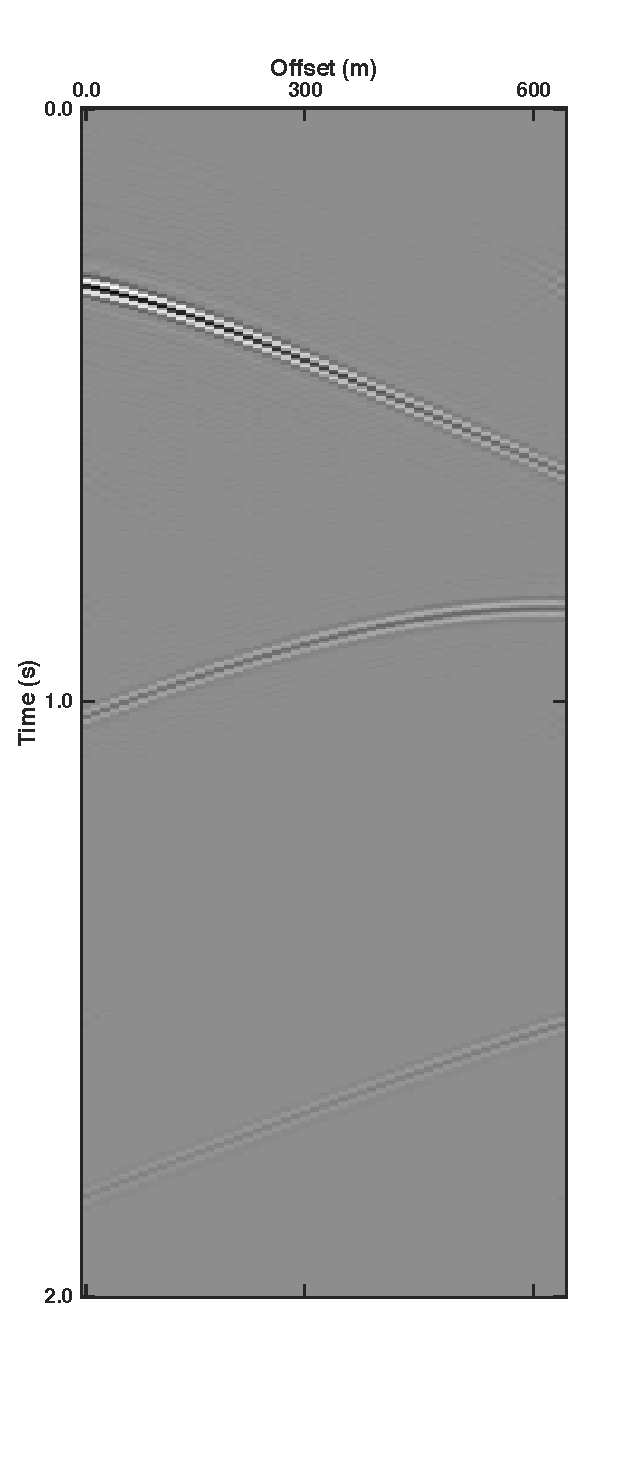
\includegraphics[height = 0.38\textheight]{Plots/BlendingPatterns/Unblended_inline10}
		\caption{}
		\label{fig:Ch-Results-Unbl-inline10}
	\end{subfigure}
	%	
	\centering
	\begin{subfigure}[t]{0.24\textwidth}
		\centering
		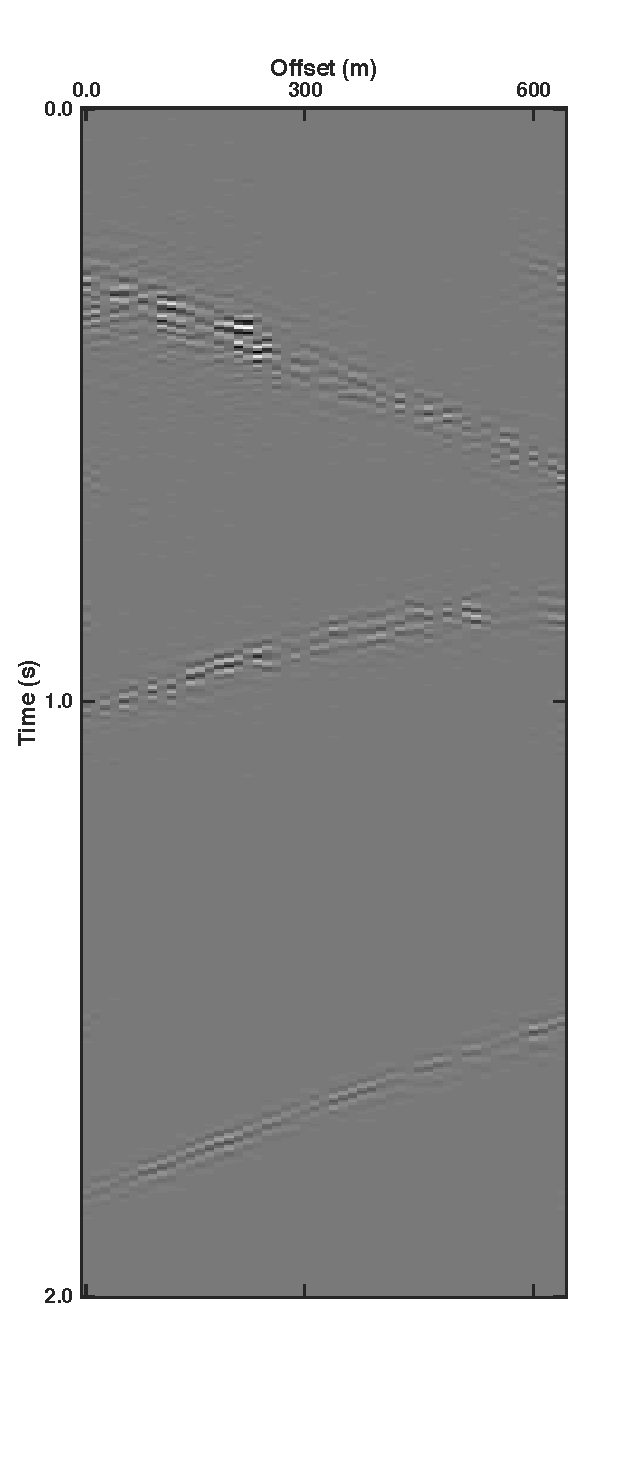
\includegraphics[height = 0.38\textheight]{Plots/BlendingPatterns/Deblended_inline10x}
		\caption{}
		\label{fig:Ch-Results-Debl-inline10-x}
	\end{subfigure}
	%
	\centering
	\begin{subfigure}[t]{0.24\textwidth}
		\centering
		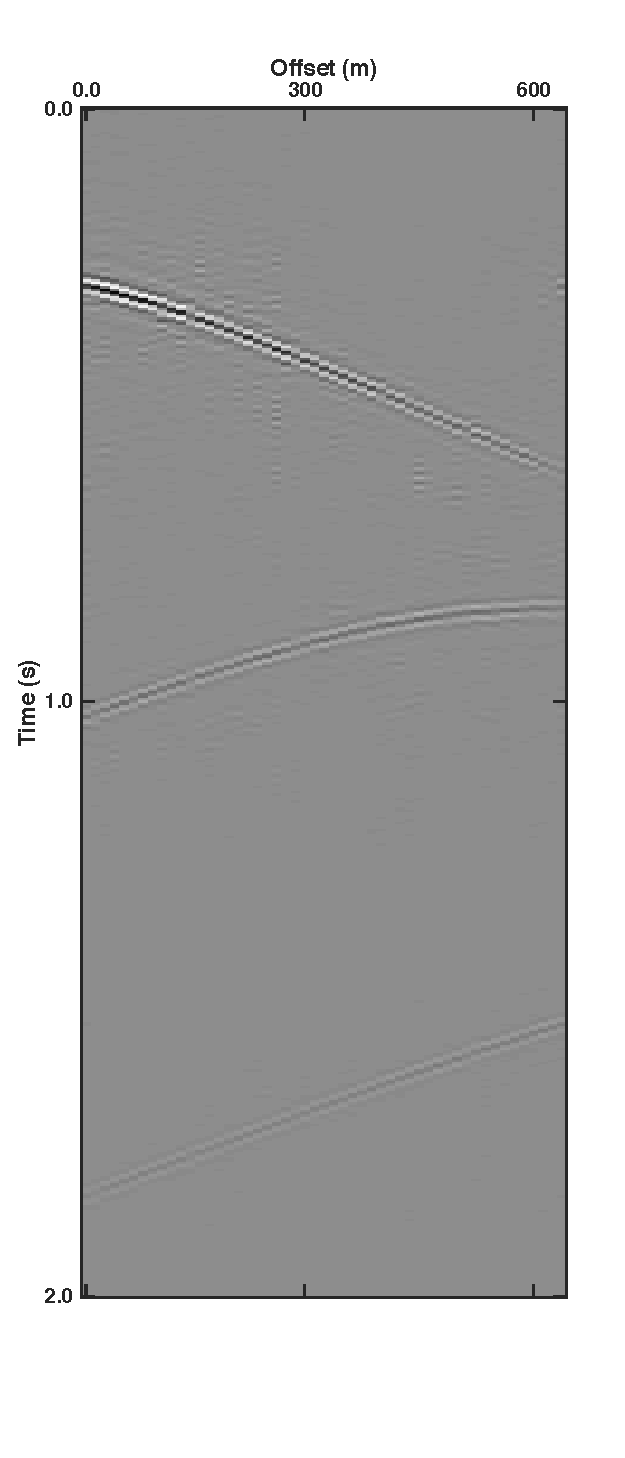
\includegraphics[height = 0.38\textheight]{Plots/BlendingPatterns/Deblended_inline10t}
		\caption{}
		\label{fig:Ch-Results-Debl-inline10-t}
	\end{subfigure}
	%
	\centering
	\begin{subfigure}[t]{0.24\textwidth}
		\centering
		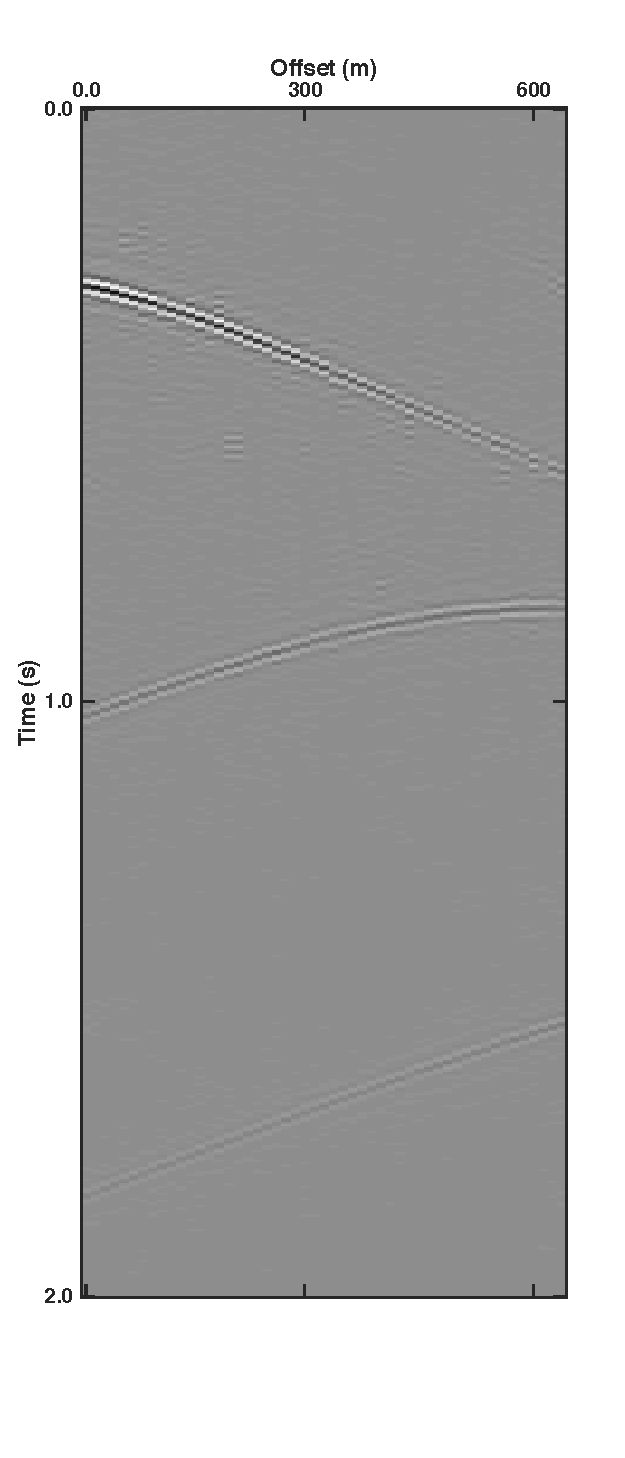
\includegraphics[height = 0.38\textheight]{Plots/BlendingPatterns/Deblended_inline10xt}
		\caption{}
		\label{fig:Ch-Results-Debl-inline10-xt}
	\end{subfigure}
	\par\bigskip
	\centering
	\begin{subfigure}[t]{0.24\textwidth}
		\centering
		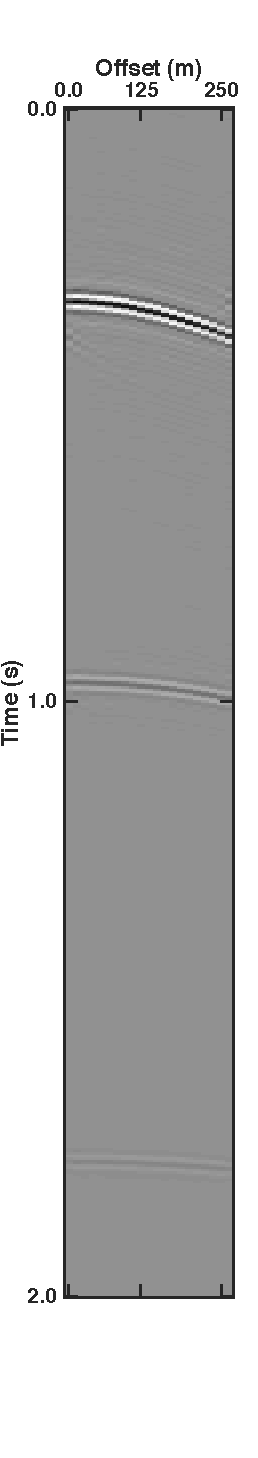
\includegraphics[height = 0.38\textheight]{Plots/BlendingPatterns/Unblended_xline10}
		\caption{}
		\label{fig:Ch-Results-Unbl-xline10}
	\end{subfigure}
	%	
	\centering
	\begin{subfigure}[t]{0.24\textwidth}
		\centering
		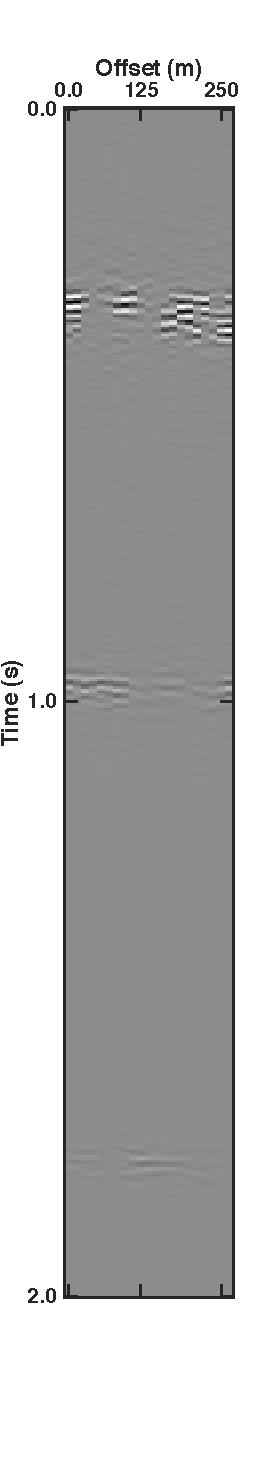
\includegraphics[height = 0.38\textheight]{Plots/BlendingPatterns/Deblended_xline10x}
		\caption{}
		\label{fig:Ch-Results-Debl-xline10-x}
	\end{subfigure}
	%
	\centering
	\begin{subfigure}[t]{0.24\textwidth}
		\centering
		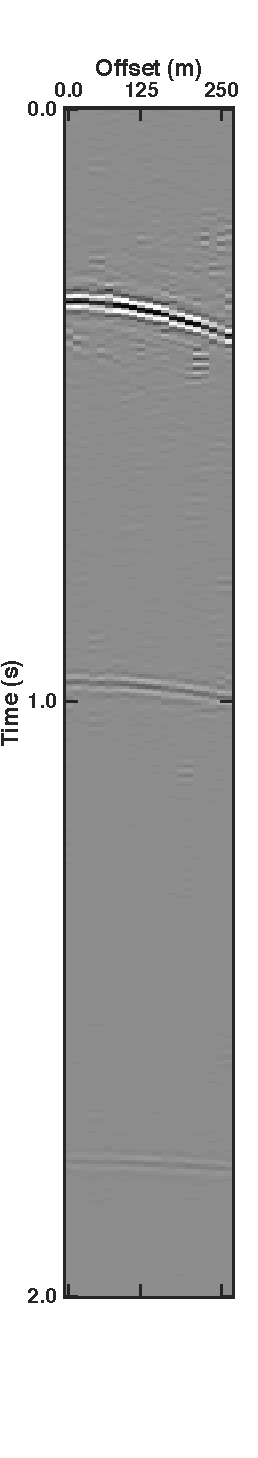
\includegraphics[height = 0.38\textheight]{Plots/BlendingPatterns/Deblended_xline10t}
		\caption{}
		\label{fig:Ch-Results-Debl-xline10-t}
	\end{subfigure}
	%
	\centering
	\begin{subfigure}[t]{0.24\textwidth}
		\centering
		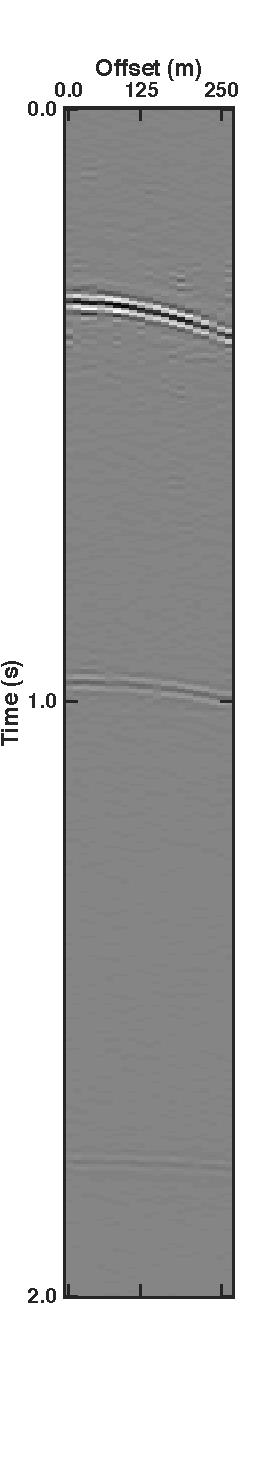
\includegraphics[height = 0.38\textheight]{Plots/BlendingPatterns/Deblended_xline10xt}
		\caption{}
		\label{fig:Ch-Results-Debl-xline10-xt}
	\end{subfigure}
	
	\caption{(a)-(d) show inline slices of the data shown in Figure \ref{fig:Ch-Results-Debl-Delphi}. (e)-(h) display the corresponding crossline slices. }
	\label{fig:Ch-Results-Debl-x-inline}

\end{figure}

The deblending performance is quantified with a quality factor, $Q$, which is defined by \citet{IbrahimQuality} as;

\begin{equation}
	Q = 10 \cdot \frac{\left|\left|\text{Unblended data}\right|\right| _2 ^2}{\left|\left|\text{Unblended data - Deblended data}\right|\right| _2 ^2} .	
\end{equation}

Figure \ref{fig:Ch-Results-QualityFactors} illustrates the quality factor for the 3 blending patterns as a function of the maximum firing time delay. The plot confirms the previous observations: Only spatial incoherency limits the deblended data quality, whereas temporal incoherency allows to achieve significantly better deblending performance. The combination of spatial and temporal incoherency can even enhance the result further.

\begin{figure}
	\centering
	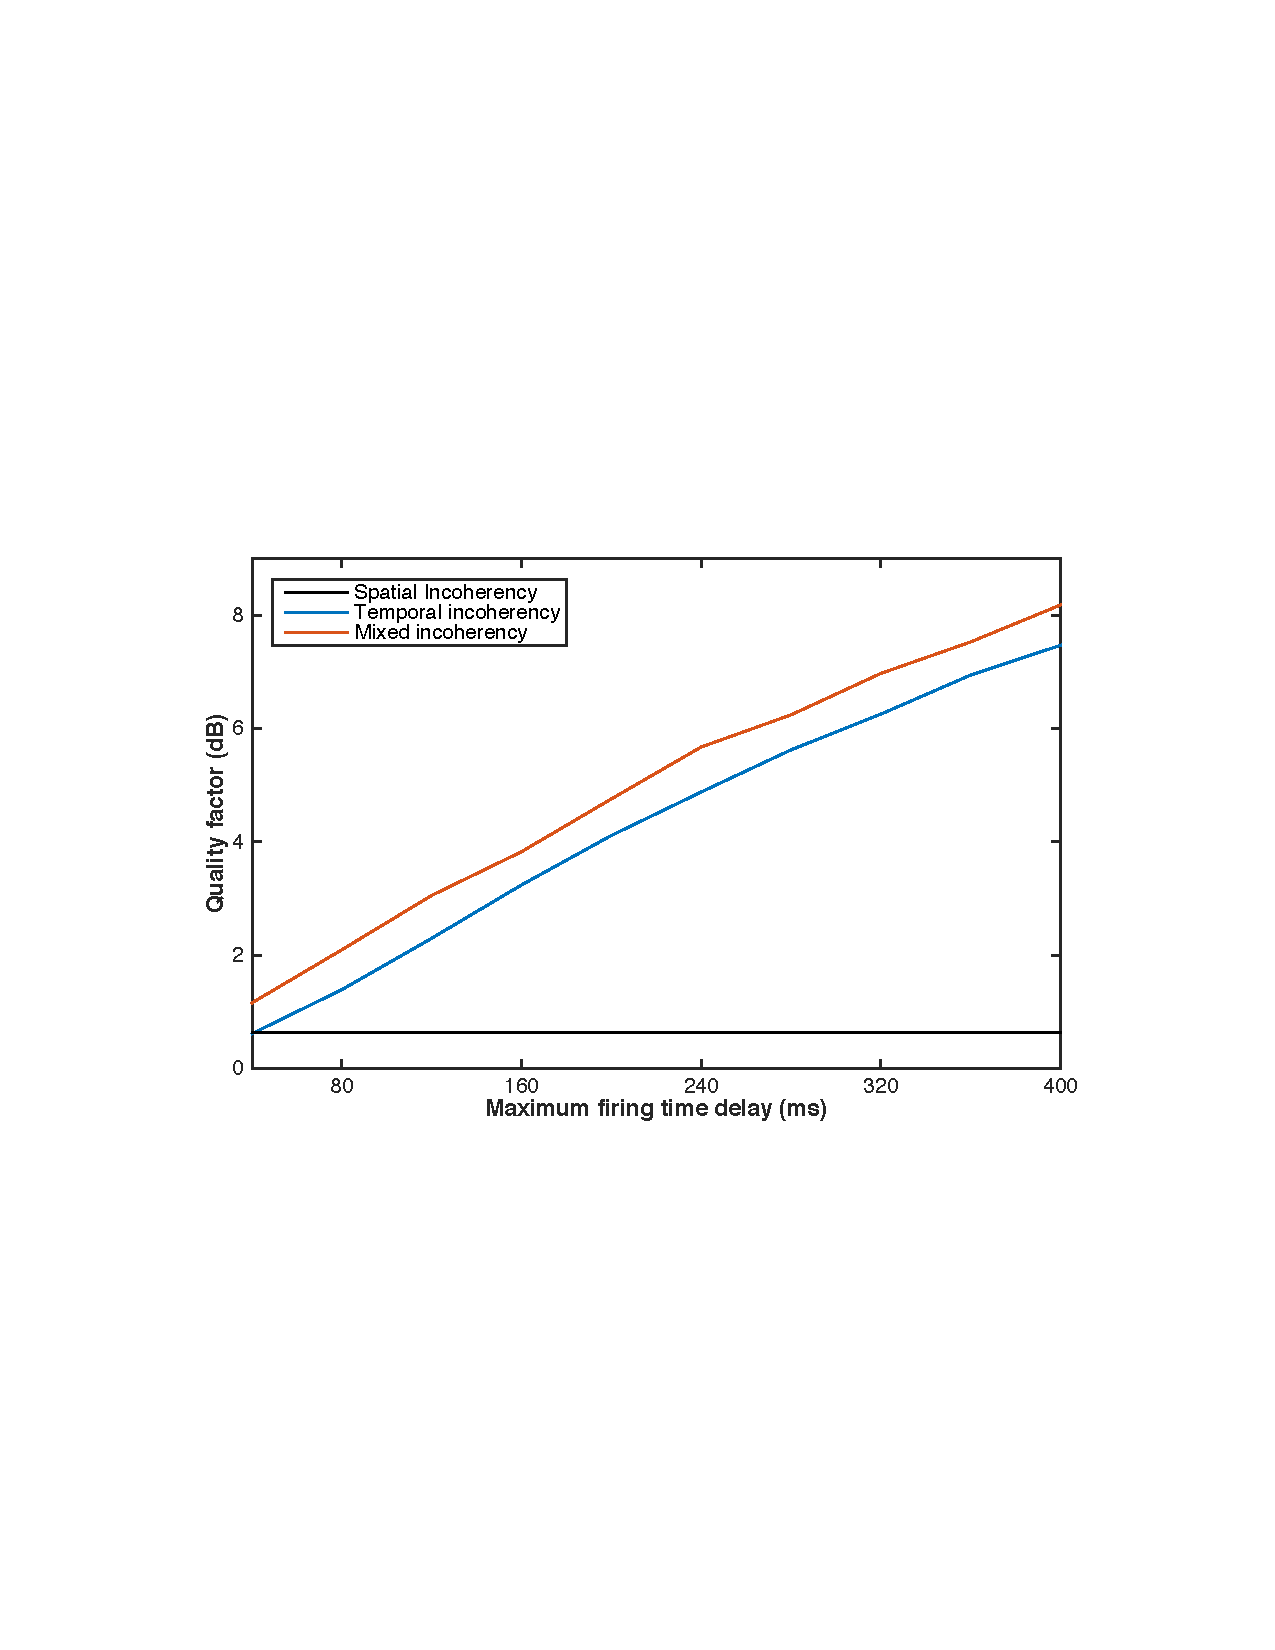
\includegraphics[width = 0.6\textwidth]{Plots/BlendingPatterns/quality_line_plot_avg}
	\caption{The 3 suggested blending patterns are simulated with maximum firing time delays between \SI{40}{\milli\second} and \SI{400}{\milli\second}. The quality factors are computed with respect to the unblended data and illustrated as a function of the maximum firing time.}
	\label{fig:Ch-Results-QualityFactors}
\end{figure}

\FloatBarrier
\section{3D FKK Filter Performance}

\section{Feasibility}








